\documentclass[]{article}
\usepackage{lmodern}
\usepackage{amssymb,amsmath}
\usepackage{ifxetex,ifluatex}
\usepackage{fixltx2e} % provides \textsubscript
\ifnum 0\ifxetex 1\fi\ifluatex 1\fi=0 % if pdftex
  \usepackage[T1]{fontenc}
  \usepackage[utf8]{inputenc}
\else % if luatex or xelatex
  \ifxetex
    \usepackage{mathspec}
  \else
    \usepackage{fontspec}
  \fi
  \defaultfontfeatures{Ligatures=TeX,Scale=MatchLowercase}
\fi
% use upquote if available, for straight quotes in verbatim environments
\IfFileExists{upquote.sty}{\usepackage{upquote}}{}
% use microtype if available
\IfFileExists{microtype.sty}{%
\usepackage{microtype}
\UseMicrotypeSet[protrusion]{basicmath} % disable protrusion for tt fonts
}{}
\usepackage[margin=1in]{geometry}
\usepackage{hyperref}
\hypersetup{unicode=true,
            pdftitle={Motor Trend Data Analysis Final Project},
            pdfauthor={Carlos Martinez Reyes},
            pdfborder={0 0 0},
            breaklinks=true}
\urlstyle{same}  % don't use monospace font for urls
\usepackage{color}
\usepackage{fancyvrb}
\newcommand{\VerbBar}{|}
\newcommand{\VERB}{\Verb[commandchars=\\\{\}]}
\DefineVerbatimEnvironment{Highlighting}{Verbatim}{commandchars=\\\{\}}
% Add ',fontsize=\small' for more characters per line
\usepackage{framed}
\definecolor{shadecolor}{RGB}{248,248,248}
\newenvironment{Shaded}{\begin{snugshade}}{\end{snugshade}}
\newcommand{\AlertTok}[1]{\textcolor[rgb]{0.94,0.16,0.16}{#1}}
\newcommand{\AnnotationTok}[1]{\textcolor[rgb]{0.56,0.35,0.01}{\textbf{\textit{#1}}}}
\newcommand{\AttributeTok}[1]{\textcolor[rgb]{0.77,0.63,0.00}{#1}}
\newcommand{\BaseNTok}[1]{\textcolor[rgb]{0.00,0.00,0.81}{#1}}
\newcommand{\BuiltInTok}[1]{#1}
\newcommand{\CharTok}[1]{\textcolor[rgb]{0.31,0.60,0.02}{#1}}
\newcommand{\CommentTok}[1]{\textcolor[rgb]{0.56,0.35,0.01}{\textit{#1}}}
\newcommand{\CommentVarTok}[1]{\textcolor[rgb]{0.56,0.35,0.01}{\textbf{\textit{#1}}}}
\newcommand{\ConstantTok}[1]{\textcolor[rgb]{0.00,0.00,0.00}{#1}}
\newcommand{\ControlFlowTok}[1]{\textcolor[rgb]{0.13,0.29,0.53}{\textbf{#1}}}
\newcommand{\DataTypeTok}[1]{\textcolor[rgb]{0.13,0.29,0.53}{#1}}
\newcommand{\DecValTok}[1]{\textcolor[rgb]{0.00,0.00,0.81}{#1}}
\newcommand{\DocumentationTok}[1]{\textcolor[rgb]{0.56,0.35,0.01}{\textbf{\textit{#1}}}}
\newcommand{\ErrorTok}[1]{\textcolor[rgb]{0.64,0.00,0.00}{\textbf{#1}}}
\newcommand{\ExtensionTok}[1]{#1}
\newcommand{\FloatTok}[1]{\textcolor[rgb]{0.00,0.00,0.81}{#1}}
\newcommand{\FunctionTok}[1]{\textcolor[rgb]{0.00,0.00,0.00}{#1}}
\newcommand{\ImportTok}[1]{#1}
\newcommand{\InformationTok}[1]{\textcolor[rgb]{0.56,0.35,0.01}{\textbf{\textit{#1}}}}
\newcommand{\KeywordTok}[1]{\textcolor[rgb]{0.13,0.29,0.53}{\textbf{#1}}}
\newcommand{\NormalTok}[1]{#1}
\newcommand{\OperatorTok}[1]{\textcolor[rgb]{0.81,0.36,0.00}{\textbf{#1}}}
\newcommand{\OtherTok}[1]{\textcolor[rgb]{0.56,0.35,0.01}{#1}}
\newcommand{\PreprocessorTok}[1]{\textcolor[rgb]{0.56,0.35,0.01}{\textit{#1}}}
\newcommand{\RegionMarkerTok}[1]{#1}
\newcommand{\SpecialCharTok}[1]{\textcolor[rgb]{0.00,0.00,0.00}{#1}}
\newcommand{\SpecialStringTok}[1]{\textcolor[rgb]{0.31,0.60,0.02}{#1}}
\newcommand{\StringTok}[1]{\textcolor[rgb]{0.31,0.60,0.02}{#1}}
\newcommand{\VariableTok}[1]{\textcolor[rgb]{0.00,0.00,0.00}{#1}}
\newcommand{\VerbatimStringTok}[1]{\textcolor[rgb]{0.31,0.60,0.02}{#1}}
\newcommand{\WarningTok}[1]{\textcolor[rgb]{0.56,0.35,0.01}{\textbf{\textit{#1}}}}
\usepackage{graphicx,grffile}
\makeatletter
\def\maxwidth{\ifdim\Gin@nat@width>\linewidth\linewidth\else\Gin@nat@width\fi}
\def\maxheight{\ifdim\Gin@nat@height>\textheight\textheight\else\Gin@nat@height\fi}
\makeatother
% Scale images if necessary, so that they will not overflow the page
% margins by default, and it is still possible to overwrite the defaults
% using explicit options in \includegraphics[width, height, ...]{}
\setkeys{Gin}{width=\maxwidth,height=\maxheight,keepaspectratio}
\IfFileExists{parskip.sty}{%
\usepackage{parskip}
}{% else
\setlength{\parindent}{0pt}
\setlength{\parskip}{6pt plus 2pt minus 1pt}
}
\setlength{\emergencystretch}{3em}  % prevent overfull lines
\providecommand{\tightlist}{%
  \setlength{\itemsep}{0pt}\setlength{\parskip}{0pt}}
\setcounter{secnumdepth}{0}
% Redefines (sub)paragraphs to behave more like sections
\ifx\paragraph\undefined\else
\let\oldparagraph\paragraph
\renewcommand{\paragraph}[1]{\oldparagraph{#1}\mbox{}}
\fi
\ifx\subparagraph\undefined\else
\let\oldsubparagraph\subparagraph
\renewcommand{\subparagraph}[1]{\oldsubparagraph{#1}\mbox{}}
\fi

%%% Use protect on footnotes to avoid problems with footnotes in titles
\let\rmarkdownfootnote\footnote%
\def\footnote{\protect\rmarkdownfootnote}

%%% Change title format to be more compact
\usepackage{titling}

% Create subtitle command for use in maketitle
\providecommand{\subtitle}[1]{
  \posttitle{
    \begin{center}\large#1\end{center}
    }
}

\setlength{\droptitle}{-2em}

  \title{Motor Trend Data Analysis Final Project}
    \pretitle{\vspace{\droptitle}\centering\huge}
  \posttitle{\par}
    \author{Carlos Martinez Reyes}
    \preauthor{\centering\large\emph}
  \postauthor{\par}
      \predate{\centering\large\emph}
  \postdate{\par}
    \date{30/10/2020}


\begin{document}
\maketitle

\hypertarget{executive-summary}{%
\section{Executive Summary}\label{executive-summary}}

In this report, we analyze the 1974 US Motor Trend magazine mtcars data
set to evaluate the effect of transmission type on MPG (miles per
gallon) performance. The database includes the fuel consumption and 10
design and performance aspects of 32 cars (1973--74 models). We use mpg
as the response variable and fit a regression model considering a set of
variables as predictors.

\hypertarget{exploratory-data-analysis}{%
\section{Exploratory Data Analysis}\label{exploratory-data-analysis}}

\begin{Shaded}
\begin{Highlighting}[]
\KeywordTok{library}\NormalTok{(ggplot2)}
\KeywordTok{data}\NormalTok{(mtcars)}
\KeywordTok{dim}\NormalTok{(mtcars)}
\end{Highlighting}
\end{Shaded}

\begin{verbatim}
## [1] 32 11
\end{verbatim}

\begin{Shaded}
\begin{Highlighting}[]
\KeywordTok{head}\NormalTok{(mtcars)}
\end{Highlighting}
\end{Shaded}

\begin{verbatim}
##                    mpg cyl disp  hp drat    wt  qsec vs am gear carb
## Mazda RX4         21.0   6  160 110 3.90 2.620 16.46  0  1    4    4
## Mazda RX4 Wag     21.0   6  160 110 3.90 2.875 17.02  0  1    4    4
## Datsun 710        22.8   4  108  93 3.85 2.320 18.61  1  1    4    1
## Hornet 4 Drive    21.4   6  258 110 3.08 3.215 19.44  1  0    3    1
## Hornet Sportabout 18.7   8  360 175 3.15 3.440 17.02  0  0    3    2
## Valiant           18.1   6  225 105 2.76 3.460 20.22  1  0    3    1
\end{verbatim}

The data consists of 32 samples (different automobiles) and 11 variables
(10 control variables, 1 target variable (mpg). The data are numeric
which is not correct for our finishers, so the next step is the
transformation of variables.

\begin{Shaded}
\begin{Highlighting}[]
\NormalTok{mtcars}\OperatorTok{$}\NormalTok{cyl \textless{}{-}}\StringTok{ }\KeywordTok{factor}\NormalTok{(mtcars}\OperatorTok{$}\NormalTok{cyl)}
\NormalTok{mtcars}\OperatorTok{$}\NormalTok{vs \textless{}{-}}\StringTok{ }\KeywordTok{factor}\NormalTok{(mtcars}\OperatorTok{$}\NormalTok{vs)}
\NormalTok{mtcars}\OperatorTok{$}\NormalTok{am \textless{}{-}}\StringTok{ }\KeywordTok{factor}\NormalTok{(mtcars}\OperatorTok{$}\NormalTok{am, }\DataTypeTok{labels =} \KeywordTok{c}\NormalTok{(}\StringTok{"Automatic"}\NormalTok{, }\StringTok{"Manual"}\NormalTok{))}
\NormalTok{mtcars}\OperatorTok{$}\NormalTok{gear \textless{}{-}}\StringTok{ }\KeywordTok{factor}\NormalTok{(mtcars}\OperatorTok{$}\NormalTok{gear)}
\NormalTok{mtcars}\OperatorTok{$}\NormalTok{carb \textless{}{-}}\StringTok{ }\KeywordTok{factor}\NormalTok{(mtcars}\OperatorTok{$}\NormalTok{carb)}
\end{Highlighting}
\end{Shaded}

Lets check the basic summary

\begin{Shaded}
\begin{Highlighting}[]
\KeywordTok{table}\NormalTok{(mtcars}\OperatorTok{$}\NormalTok{am)}
\end{Highlighting}
\end{Shaded}

\begin{verbatim}
## 
## Automatic    Manual 
##        19        13
\end{verbatim}

\begin{Shaded}
\begin{Highlighting}[]
\KeywordTok{aggregate}\NormalTok{(mpg }\OperatorTok{\textasciitilde{}}\StringTok{ }\NormalTok{am, }\DataTypeTok{data =}\NormalTok{ mtcars, mean)}
\end{Highlighting}
\end{Shaded}

\begin{verbatim}
##          am      mpg
## 1 Automatic 17.14737
## 2    Manual 24.39231
\end{verbatim}

From the above we can see that the automatic type car travels less miles
per gallon compared to the manual transmission and this is also
confirmed visually by referring to the FIGURE 1 in the appendix where we
can see in the box diagram that the manual transmission provides a
better MPG overall.

\hypertarget{statistical-inference}{%
\section{Statistical inference}\label{statistical-inference}}

From the above we can say that ON AVERAGE the automatic type travels
less miles per gallon compared to the manual transmission and we also
confirm this analytically by proving that the difference between the MPG
averages is statistically significant (Null hypothesis: the difference
is not significant). We use the two-sample T-test to prove it.

\begin{Shaded}
\begin{Highlighting}[]
\NormalTok{Auto \textless{}{-}}\StringTok{ }\NormalTok{mtcars[mtcars}\OperatorTok{$}\NormalTok{am }\OperatorTok{==}\StringTok{ "Automatic"}\NormalTok{,]}\OperatorTok{$}\NormalTok{mpg}
\NormalTok{NonAuto \textless{}{-}}\StringTok{ }\NormalTok{mtcars[mtcars}\OperatorTok{$}\NormalTok{am }\OperatorTok{==}\StringTok{ "Manual"}\NormalTok{,]}\OperatorTok{$}\NormalTok{mpg}
\KeywordTok{t.test}\NormalTok{(Auto, NonAuto)}
\end{Highlighting}
\end{Shaded}

\begin{verbatim}
## 
##  Welch Two Sample t-test
## 
## data:  Auto and NonAuto
## t = -3.7671, df = 18.332, p-value = 0.001374
## alternative hypothesis: true difference in means is not equal to 0
## 95 percent confidence interval:
##  -11.280194  -3.209684
## sample estimates:
## mean of x mean of y 
##  17.14737  24.39231
\end{verbatim}

\hypertarget{quantifying-the-mean}{%
\subsubsection{Quantifying the Mean}\label{quantifying-the-mean}}

Since the p-value is 0.001374, we reject the null hypothesis at 5\% and
1\% significance level and the mean MPG of cars with manual transmission
is different (7.245 times more) from the average performance of cars
with automatic transmission.

\hypertarget{regression-analysis}{%
\section{Regression Analysis}\label{regression-analysis}}

We have already tested that there is a significant difference at 5\% and
1\% in the average MPG performance and we roughly quantify this
difference. Now let's see what kind of relationship the MPG variable has
with the rest of the factors. We will fit three regression models to the
data to see if there is any change in mpg based on the transmission and
we will see how the transmission affects the mpg by considering other
variables.

\hypertarget{model-1-mpg-and-transmission}{%
\subsection{Model 1: MPG and
Transmission}\label{model-1-mpg-and-transmission}}

Here we start with a very simple model that is mpg regressed by am -
Transmission.

\begin{Shaded}
\begin{Highlighting}[]
\NormalTok{fitam \textless{}{-}}\StringTok{ }\KeywordTok{lm}\NormalTok{(mpg }\OperatorTok{\textasciitilde{}}\StringTok{ }\NormalTok{am, mtcars)}
\KeywordTok{summary}\NormalTok{(fitam)}
\end{Highlighting}
\end{Shaded}

\begin{verbatim}
## 
## Call:
## lm(formula = mpg ~ am, data = mtcars)
## 
## Residuals:
##     Min      1Q  Median      3Q     Max 
## -9.3923 -3.0923 -0.2974  3.2439  9.5077 
## 
## Coefficients:
##             Estimate Std. Error t value Pr(>|t|)    
## (Intercept)   17.147      1.125  15.247 1.13e-15 ***
## amManual       7.245      1.764   4.106 0.000285 ***
## ---
## Signif. codes:  0 '***' 0.001 '**' 0.01 '*' 0.05 '.' 0.1 ' ' 1
## 
## Residual standard error: 4.902 on 30 degrees of freedom
## Multiple R-squared:  0.3598, Adjusted R-squared:  0.3385 
## F-statistic: 16.86 on 1 and 30 DF,  p-value: 0.000285
\end{verbatim}

The R2 value for this model is only 0.3598, which means that adjusting
mpg only with am explains about 36\% of the variation in mpg because of
its linear relationship. From the model we get an adjusted R-squared of
33.85\% this quite a low variance explained by the model. Due to little
variance explained by the model let examine other variable that are
might be relevent to explain more variance to build a multivariate
linear regression. Building a model that regresses mpg on all other
variables in the dataset will explain more of the variance.

\hypertarget{model-2-mpg-and-all-variables}{%
\subsection{Model 2: MPG and all
Variables}\label{model-2-mpg-and-all-variables}}

\begin{Shaded}
\begin{Highlighting}[]
\NormalTok{fullmodel \textless{}{-}}\StringTok{ }\KeywordTok{lm}\NormalTok{(mpg }\OperatorTok{\textasciitilde{}}\StringTok{ }\NormalTok{., mtcars)}
\KeywordTok{summary}\NormalTok{(fullmodel)}
\end{Highlighting}
\end{Shaded}

\begin{verbatim}
## 
## Call:
## lm(formula = mpg ~ ., data = mtcars)
## 
## Residuals:
##     Min      1Q  Median      3Q     Max 
## -3.5087 -1.3584 -0.0948  0.7745  4.6251 
## 
## Coefficients:
##             Estimate Std. Error t value Pr(>|t|)  
## (Intercept) 23.87913   20.06582   1.190   0.2525  
## cyl6        -2.64870    3.04089  -0.871   0.3975  
## cyl8        -0.33616    7.15954  -0.047   0.9632  
## disp         0.03555    0.03190   1.114   0.2827  
## hp          -0.07051    0.03943  -1.788   0.0939 .
## drat         1.18283    2.48348   0.476   0.6407  
## wt          -4.52978    2.53875  -1.784   0.0946 .
## qsec         0.36784    0.93540   0.393   0.6997  
## vs1          1.93085    2.87126   0.672   0.5115  
## amManual     1.21212    3.21355   0.377   0.7113  
## gear4        1.11435    3.79952   0.293   0.7733  
## gear5        2.52840    3.73636   0.677   0.5089  
## carb2       -0.97935    2.31797  -0.423   0.6787  
## carb3        2.99964    4.29355   0.699   0.4955  
## carb4        1.09142    4.44962   0.245   0.8096  
## carb6        4.47757    6.38406   0.701   0.4938  
## carb8        7.25041    8.36057   0.867   0.3995  
## ---
## Signif. codes:  0 '***' 0.001 '**' 0.01 '*' 0.05 '.' 0.1 ' ' 1
## 
## Residual standard error: 2.833 on 15 degrees of freedom
## Multiple R-squared:  0.8931, Adjusted R-squared:  0.779 
## F-statistic:  7.83 on 16 and 15 DF,  p-value: 0.000124
\end{verbatim}

As expected, the full model has a higher R2 value (0.8931). But the
output of summary shows that none of the coefficients are significant at
the 0.05 level. Including all the variables as the model has improved
that is by explaining 77.9\% of the variance which is given by Adjusted
R-squared. The model has a residual standard error of 2.83, which means
that the difference between the actual mpg and predicted mpg in the
model differ by about 2.82 percentage points. We also get an R-squared
of 0.8931.

\hypertarget{model-3-bestfit}{%
\subsection{Model 3: BESTFIT}\label{model-3-bestfit}}

From figure 2 of the appendix we can see that there are predictor
variables correlated with the am factor, which is why the exclusion of
the variables that are correlated with the type of transmission is
justified and will introduce biases in the coefficients. However,
including unnecessary regressors will inflate the variance of the model.

\begin{Shaded}
\begin{Highlighting}[]
\NormalTok{bestfit \textless{}{-}}\StringTok{ }\KeywordTok{lm}\NormalTok{(mpg }\OperatorTok{\textasciitilde{}}\StringTok{ }\NormalTok{cyl }\OperatorTok{+}\StringTok{ }\NormalTok{hp }\OperatorTok{+}\StringTok{ }\NormalTok{wt }\OperatorTok{+}\StringTok{ }\NormalTok{qsec }\OperatorTok{+}\StringTok{ }\NormalTok{am, }\DataTypeTok{data =}\NormalTok{ mtcars)}
\KeywordTok{summary}\NormalTok{(bestfit)}
\end{Highlighting}
\end{Shaded}

\begin{verbatim}
## 
## Call:
## lm(formula = mpg ~ cyl + hp + wt + qsec + am, data = mtcars)
## 
## Residuals:
##     Min      1Q  Median      3Q     Max 
## -3.9511 -1.4244 -0.1767  1.3666  4.2187 
## 
## Coefficients:
##             Estimate Std. Error t value Pr(>|t|)   
## (Intercept) 21.57617   11.27271   1.914   0.0671 . 
## cyl6        -1.90950    1.72992  -1.104   0.2802   
## cyl8        -0.22716    2.87047  -0.079   0.9376   
## hp          -0.02481    0.01515  -1.637   0.1141   
## wt          -2.96274    0.97728  -3.032   0.0056 **
## qsec         0.61917    0.55987   1.106   0.2793   
## amManual     2.83270    1.67020   1.696   0.1023   
## ---
## Signif. codes:  0 '***' 0.001 '**' 0.01 '*' 0.05 '.' 0.1 ' ' 1
## 
## Residual standard error: 2.4 on 25 degrees of freedom
## Multiple R-squared:  0.8721, Adjusted R-squared:  0.8414 
## F-statistic: 28.42 on 6 and 25 DF,  p-value: 5.196e-10
\end{verbatim}

This works as expected the model has improved significantly to attain a
R-squared of 84.14\% and reduced our residual standard error to 2.4 from
2.8.

\hypertarget{anova}{%
\subsubsection{ANOVA}\label{anova}}

Here run an anova test between the three models to see if they are
significantly different from one another. anova(fitam, fullmodel,
bestfit)

This results in a p-value of 2.886e-05, and we can claim the bestfit
model is significantly better and can see they are all normally
distributed and homoskedastic.(see Figure 3)

\hypertarget{residuals-normality-test}{%
\subsubsection{Residuals Normality
Test}\label{residuals-normality-test}}

\hypertarget{shapiro-wikes-test.}{%
\paragraph{Shapiro-Wikes Test.}\label{shapiro-wikes-test.}}

However, this evaluation of residuals is based on the assumption of
normality of residuals. A simple Shapiro-Wilkes test should confirm or
negate this assumption.

\begin{Shaded}
\begin{Highlighting}[]
\NormalTok{Sfit=}\KeywordTok{shapiro.test}\NormalTok{(fitam}\OperatorTok{$}\NormalTok{resid)}
\KeywordTok{print}\NormalTok{(Sfit)}
\end{Highlighting}
\end{Shaded}

\begin{verbatim}
## 
##  Shapiro-Wilk normality test
## 
## data:  fitam$resid
## W = 0.98208, p-value = 0.8573
\end{verbatim}

\begin{Shaded}
\begin{Highlighting}[]
\NormalTok{Sfull=}\KeywordTok{shapiro.test}\NormalTok{(fullmodel}\OperatorTok{$}\NormalTok{resid)}
\KeywordTok{print}\NormalTok{(Sfull)}
\end{Highlighting}
\end{Shaded}

\begin{verbatim}
## 
##  Shapiro-Wilk normality test
## 
## data:  fullmodel$resid
## W = 0.96146, p-value = 0.301
\end{verbatim}

\begin{Shaded}
\begin{Highlighting}[]
\NormalTok{Sbest=}\KeywordTok{shapiro.test}\NormalTok{(bestfit}\OperatorTok{$}\NormalTok{resid)}
\KeywordTok{print}\NormalTok{(Sbest)}
\end{Highlighting}
\end{Shaded}

\begin{verbatim}
## 
##  Shapiro-Wilk normality test
## 
## data:  bestfit$resid
## W = 0.96809, p-value = 0.4484
\end{verbatim}

From the outputs, in all cases the p-value \textgreater{} 0.05 implying
that the distribution of the data are not significantly different from
normal distribution. In other words, we can assume the normality. Hence,
our evaluation of the residuals is valid and the models are a good fit
for the data. This is supported by the graphs in Figure 3.

\hypertarget{appendix}{%
\subsection{Appendix}\label{appendix}}

\hypertarget{figure-1.}{%
\subsubsection{Figure 1.}\label{figure-1.}}

\begin{Shaded}
\begin{Highlighting}[]
\KeywordTok{boxplot}\NormalTok{(mtcars}\OperatorTok{$}\NormalTok{mpg}\OperatorTok{\textasciitilde{}}\KeywordTok{factor}\NormalTok{(mtcars}\OperatorTok{$}\NormalTok{am, }\DataTypeTok{labels=}\KeywordTok{c}\NormalTok{(}\StringTok{"Automatic"}\NormalTok{, }\StringTok{"Manual"}\NormalTok{)),}
\DataTypeTok{col=}\KeywordTok{c}\NormalTok{(}\StringTok{"lightblue"}\NormalTok{, }\StringTok{"orange"}\NormalTok{), }\DataTypeTok{xlab=}\StringTok{"Transmission type"}\NormalTok{,}
\DataTypeTok{ylab=}\StringTok{"Mean MPG"}\NormalTok{)}
\end{Highlighting}
\end{Shaded}

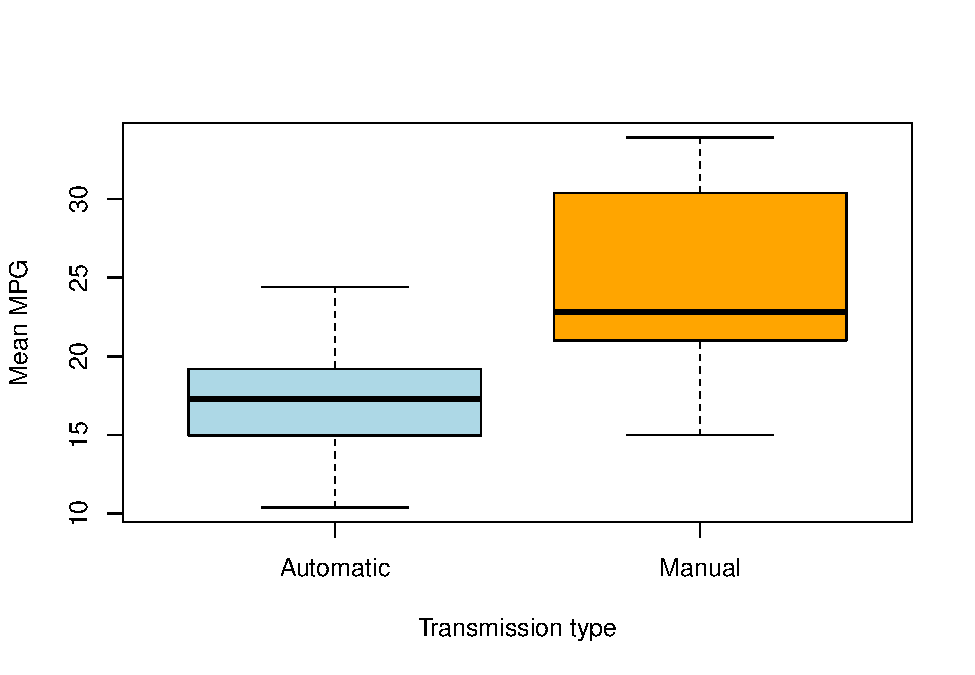
\includegraphics{Motor_Trend_Data_Analysis_Final_Project_files/figure-latex/unnamed-chunk-9-1.pdf}
Lo que muestra el gráfico corresponde a la prueba t realizada
anteriormente.

\hypertarget{figure-2.}{%
\subsubsection{Figure 2.}\label{figure-2.}}

\begin{Shaded}
\begin{Highlighting}[]
\KeywordTok{library}\NormalTok{(reshape2)}
\KeywordTok{library}\NormalTok{(ggplot2)}
\KeywordTok{data}\NormalTok{(mtcars)}
\KeywordTok{dim}\NormalTok{(mtcars)}
\end{Highlighting}
\end{Shaded}

\begin{verbatim}
## [1] 32 11
\end{verbatim}

\begin{Shaded}
\begin{Highlighting}[]
\KeywordTok{head}\NormalTok{(mtcars)}
\end{Highlighting}
\end{Shaded}

\begin{verbatim}
##                    mpg cyl disp  hp drat    wt  qsec vs am gear carb
## Mazda RX4         21.0   6  160 110 3.90 2.620 16.46  0  1    4    4
## Mazda RX4 Wag     21.0   6  160 110 3.90 2.875 17.02  0  1    4    4
## Datsun 710        22.8   4  108  93 3.85 2.320 18.61  1  1    4    1
## Hornet 4 Drive    21.4   6  258 110 3.08 3.215 19.44  1  0    3    1
## Hornet Sportabout 18.7   8  360 175 3.15 3.440 17.02  0  0    3    2
## Valiant           18.1   6  225 105 2.76 3.460 20.22  1  0    3    1
\end{verbatim}

\begin{Shaded}
\begin{Highlighting}[]
\NormalTok{data=}\StringTok{ }\NormalTok{mtcars}
\NormalTok{corheatmap =}\StringTok{ }\KeywordTok{round}\NormalTok{(}\KeywordTok{cor}\NormalTok{(data),}\DecValTok{2}\NormalTok{)}
\NormalTok{corheatmap[}\KeywordTok{lower.tri}\NormalTok{(corheatmap)]\textless{}{-}}\StringTok{ }\OtherTok{NA}
\NormalTok{melted \textless{}{-}}\StringTok{ }\KeywordTok{melt}\NormalTok{(corheatmap)}
\NormalTok{melted \textless{}{-}}\StringTok{ }\KeywordTok{na.omit}\NormalTok{(melted)}
\KeywordTok{ggplot}\NormalTok{(}\DataTypeTok{data =}\NormalTok{ melted, }\KeywordTok{aes}\NormalTok{(Var2, Var1, }\DataTypeTok{fill =}\NormalTok{ value))}\OperatorTok{+}
\KeywordTok{ggtitle}\NormalTok{(}\StringTok{"Correlation Heatmap"}\NormalTok{)}\OperatorTok{+}
\KeywordTok{geom\_tile}\NormalTok{(}\DataTypeTok{color =} \StringTok{"white"}\NormalTok{)}\OperatorTok{+}
\KeywordTok{scale\_fill\_gradient2}\NormalTok{(}\DataTypeTok{low =} \StringTok{"blue"}\NormalTok{,}
\DataTypeTok{high =} \StringTok{"red"}\NormalTok{, }\DataTypeTok{mid =} \StringTok{"white"}\NormalTok{,}
\DataTypeTok{midpoint =} \DecValTok{0}\NormalTok{, }\DataTypeTok{limit =} \KeywordTok{c}\NormalTok{(}\OperatorTok{{-}}\DecValTok{1}\NormalTok{,}\DecValTok{1}\NormalTok{), }\DataTypeTok{name=}\StringTok{"Correlation"}\NormalTok{)}\OperatorTok{+}
\KeywordTok{theme\_minimal}\NormalTok{()}\OperatorTok{+}\KeywordTok{coord\_fixed}\NormalTok{()}
\end{Highlighting}
\end{Shaded}

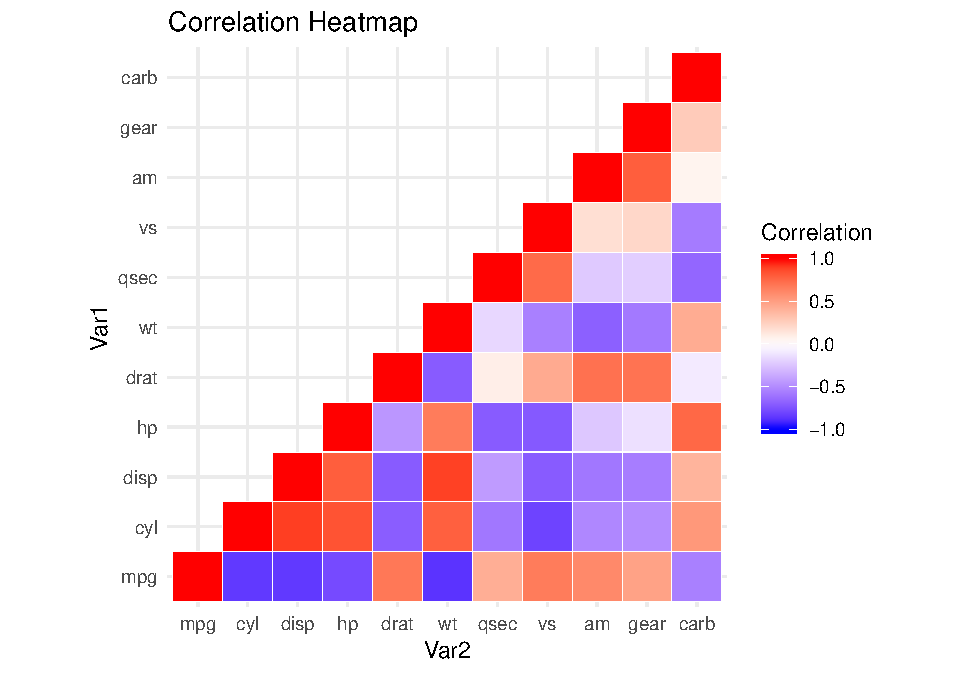
\includegraphics{Motor_Trend_Data_Analysis_Final_Project_files/figure-latex/unnamed-chunk-11-1.pdf}

Variables correlated.

\hypertarget{figure-3.}{%
\subsubsection{Figure 3.}\label{figure-3.}}

\begin{Shaded}
\begin{Highlighting}[]
\KeywordTok{par}\NormalTok{(}\DataTypeTok{mfrow =} \KeywordTok{c}\NormalTok{(}\DecValTok{2}\NormalTok{,}\DecValTok{2}\NormalTok{))}
\KeywordTok{plot}\NormalTok{(bestfit, }\DataTypeTok{col =} \StringTok{"blue"}\NormalTok{, }\DataTypeTok{lwd =} \DecValTok{2}\NormalTok{)}
\end{Highlighting}
\end{Shaded}

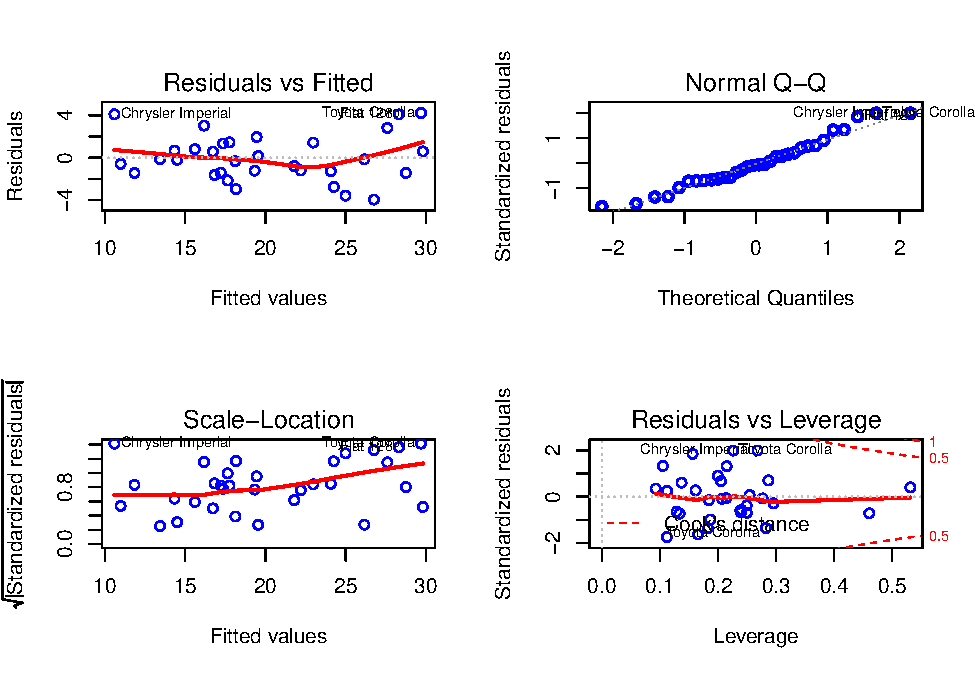
\includegraphics{Motor_Trend_Data_Analysis_Final_Project_files/figure-latex/unnamed-chunk-12-1.pdf}

The Residual Fit Plot looks how we would expect it to look if residuals
were independently and almost identically distributed with zero mean,
and were uncorrelated with the fit. The highest residuals were for the
outliers. The QQ Plot shows how the outliers, the Chrysler Impala, Lotus
Europa and Fiat 128 affect the curve. Although they change the
regression model, their impact is important and it would be unwise to
remove them.

\hypertarget{conclusions}{%
\subsection{Conclusions}\label{conclusions}}

Collectively for all control variables considered together, there is
significant effect, while for each control variable including
transmission design effect is insignificant. Individually, transmission
design shows significant difference on MPG.


\end{document}
